\section{Torsion in pretzel links}
\label{sec:computation}

\definecolor{pretzelcol1}{rgb}{0.8,0,0.3}
\definecolor{pretzelcol2}{rgb}{0.3,0,0.8}

\NewDocumentCommand{\respretzel}{O{0}O{0}O{1}O{1}O{1}}{
  \ifnum#3=0
    \webid[#1-1][#2-2.5]
  \else
    \webs[#1-1][#2-2.5]\webm[#1][#2-2.5]
  \fi
  \ifnum#4=0
    \webid[#1-1][#2-.5]
  \else
    \webs[#1-1][#2-.5]\webm[#1][#2-.5]
  \fi
  \ifnum#5=0
    \webid[#1-1][#2+1.5]
  \else
    \webs[#1-1][#2+1.5]\webm[#1][#2+1.5]
  \fi
  %
  \draw[web1] (#1-1,#2-1.5) to[out=180,in=180] (#1-1,#2-.5);
  \draw[web1] (#1-1,#2+.5) to[out=180,in=180] (#1-1,#2+1.5);
  \draw[web1] (#1-1,#2-2.5) to[out=180,in=180] (#1-1,#2+2.5);
  \draw[web1] (#1+1,#2-1.5) to[out=0,in=0] (#1+1,#2-.5);
  \draw[web1] (#1+1,#2+.5) to[out=0,in=0] (#1+1,#2+1.5);
  \draw[web1] (#1+1,#2-2.5) to[out=0,in=0] (#1+1,#2+2.5);
}

\tikzset{gaussmark/.style={circle,fill=white,draw=black,line width=.5pt,inner sep=1pt}}

In this section, we partially compute the odd Khovanov homology of the pretzel links $P(n,n,-n)$ and prove \cref{thm:main_pretzel}.

First, we take advantage of the extension to tangles, and compute the $n$th crossing twist:

\begin{lemma}
  \label{lem:n-crossing-twist}
  \def\webscl{.3}
  \def\intspc{5mu}
  Let $n\in\bN$.
  The following are isomorphisms in the relative homology category $\cK^{\gloo}(\sfoam^{\greenmarking})$ (the wiggly lines indicate homological degree zero):
  \begin{gather*}
    \scriptstyle
    \underbrace{
    \tikzpic{
      \webncr
      \node at (2,.5) {$\ldots$};
      \webncr[3][0]
    }[scale=\webscl][(0,.5*\webscl)]
    }_n
    %
    \quad\simeq^{\gloo}\quad
    %
    \tikzpic{
      \websRoundMarkedB[0][0][]
      \webm[1][0]
    }[scale=\webscl][(0,.5*\webscl)]
    \;\langle-\frac{n}{2},\frac{n}{2}\rangle
    %
    \mspace{\intspc}
    \xrightarrow{
      \tikzpic{\frst\flst[1][0]\fdot[-.7][.5]}[scale=.4,xscale=.5]
      \;-\;
      \tikzpic{\frst\flst[1][0]\fdot[1.7][.5]}[scale=.4,xscale=.5]
    }
    \mspace{\intspc}
    %
    \tikzpic{
      \websRoundMarkedB[0][0][]
      \webm[1][0]
    }[scale=\webscl][(0,.5*\webscl)]
    \;\langle-\frac{(n-1)}{2},\frac{(n-1)}{2}\rangle
    %
    \mspace{\intspc}
    {\textstyle \ldots}
    \mspace{\intspc}
    \xrightarrow{
      \tikzpic{\frst\flst[1][0]\fdot[-.7][.5]}[scale=.4,xscale=.5]
      \;-\;
      \tikzpic{\frst\flst[1][0]\fdot[1.7][.5]}[scale=.4,xscale=.5]
    }
    \mspace{\intspc}
    %
    \tikzpic{
      \websRoundMarkedB[0][0][]
      \webm[1][0]
    }[scale=\webscl][(0,.5*\webscl)]
    \;\langle-\frac{1}{2},\frac{1}{2}\rangle
    %
    \mspace{\intspc}
    \xrightarrow{\tikzpic{\funzip}[scale=.4,xscale=.7]}
    \mspace{\intspc}
    %
    \tikzpic{
      \webid
      \draw[decorate,decoration=snake] (0,-.5) to (2,-.5);
    }[scale=\webscl][(0,.5*\webscl)]
    \\[2ex]
    %%%%%%%%%%%%%%%%%%%%%%%%%%%%%%
    %%%%%%%%%%%%%%%%%%%%%%%%%%%%%%
    \scriptstyle
    \underbrace{
    \tikzpic{
      \webpcr
      \node at (2,.5) {$\ldots$};
      \webpcr[3][0]
    }[scale=\webscl][(0,.5*\webscl)]
    }_n
    %
    \quad\simeq^{\gloo}\quad
    %
    \tikzpic{
      \webid
    }[scale=\webscl][(0,.5*\webscl)]
    \;\langle-\frac{n}{2},\frac{n}{2}\rangle
    %
    \mspace{\intspc}
    \xrightarrow{\tikzpic{\fzip}[scale=.4,xscale=.7]}
    \mspace{\intspc}
    %
    \tikzpic{
      \websRoundMarkedB[0][0][]
      \webm[1][0]
    }[scale=\webscl][(0,.5*\webscl)]
    \;\langle-\frac{(n-1)}{2},\frac{(n-1)}{2}\rangle
    %
    \mspace{\intspc}
    \xrightarrow{
      \tikzpic{\frst\flst[1][0]\fdot[-.7][.5]}[scale=.4,xscale=.5]
      \;-\;
      \tikzpic{\frst\flst[1][0]\fdot[1.7][.5]}[scale=.4,xscale=.5]
    }
    %
    \mspace{\intspc}
    {\textstyle \ldots}
    \mspace{\intspc}
    %
    \tikzpic{
      \websRoundMarkedB[0][0][]
      \webm[1][0]
    }[scale=\webscl][(0,.5*\webscl)]
    \;\langle-\frac{1}{2},\frac{1}{2}\rangle
    %
    \mspace{\intspc}
    \xrightarrow{
      \tikzpic{\frst\flst[1][0]\fdot[-.7][.5]}[scale=.4,xscale=.5]
      \;-\;
      \tikzpic{\frst\flst[1][0]\fdot[1.7][.5]}[scale=.4,xscale=.5]
    }
    \mspace{\intspc}
    %
    \tikzpic{
      \websRoundMarkedB[0][0][]
      \webm[1][0]
      \draw[decorate,decoration=snake] (0,-.5) to (2,-.5);
    }[scale=\webscl][(0,.5*\webscl)]
  \end{gather*}
\end{lemma}

\begin{proof}
  This can be shown by induction.
  Resolving the last crossing expresses the right-hand side as a cone over an equivariant chain morphism $f$.
  On the one hand, using the deformation retracts given in the proof of invariance under Reidemeister I (\cref{lem:invariance_Reidemeister_I}), one can simplify the source (resp.\ the target) of $f$;
  on the other hand, the target (resp.\ source) can be simplified using induction.
  This concludes.
\end{proof}

From now on, we ignore gradings.

The preztel link $P(n,n,-n)$ has three ``crossing bridges''; given \cref{lem:n-crossing-twist}, the associated complex can be identified with an $(n+1)\times (n+1)\times (n+1)$ hypercube.
Two slices of this hypercube are depicted in \cref{subfig:preztel_3_square_resolutions}, in the case $n=3$.
They correspond to fixing a resolution for the bottom crossing bridge.

To proceed, we work with state spaces; that is, we apply a representable functor as in \cref{thm:equivalence_local_global}. Furthermore, we restrict to reduced odd Khovanov homology; see \cref{lem:action_on_reduced}.
This means that if a state has $k$ circles, its associated state space is $2^{k-1}$-dimensional.
\Cref{subfig:pretzel_3_schematic} gives a schematic of the $4\times 4\times 4$ hypercube associated to $P(3,3,-3)$, for a suitable choice of basis elements in each state space. One recognizes the four slices of the hypercube, given by fixing a resolution for the bottom crossing bridge; the first slice corresponds to the first slice in \cref{subfig:preztel_3_square_resolutions}, while the other slices correspond to the second slice in \cref{subfig:preztel_3_square_resolutions}.
Each point is a basis element, or rather the copy of $\bZ$ it generates, and each (dashed) line is (minus) an identity, always reading from left to right.
For instance, here are the basis elements for the following state space (here $\omega=(1,\frac{1}{2},\frac{1}{2})$):
\begin{gather*}
  \Hom_{\sfoam^{\greenmarking}}\left(\emptyset,
   \tikzpic{
    \respretzel[0][0][1][1][1]
    \node[green_mark] at (-2,2) {};
    \node[left=-1pt] at (-2,2) {\scriptsize $\omega$};
    \node[green_mark] at (2,2) {};
    \node[right=-1pt] at (2,2) {\scriptsize $-\omega$};
  }[scale=.18]\right)\cong\langle 1,t\rangle_{\ringfoam}
  \quad\text{depicted as}\quad
  \tikzpic{
    \node[fill=black,circle,inner sep=1pt] at (0,0) {};
    \node[left] at (0,0) {$1$};
    \node[fill=black,circle,inner sep=1pt] at (0,1) {};
    \node[left] at (0,1) {$t$};
    \draw[thick,red,->] (0,0) to[out=0,in=-90] (.5,.5) to[out=90,in=0] (0,1);
  }\;.
\end{gather*}
More explicitly, the isomorphism is given as follows.
Let $W$ be the state and $\beta^W$ an undotted cup foam for $W$ (see \cref{subsec:comparison_local_global}).
Let $\id_W^L$ (resp.\ $\id_W^R$) be the identity of $W$ with an additional dot on the thickening of the left (resp.\ right) circle. Then the isomorphism identifies $\beta^W\leftrightarrow 1$ and $(\id_W^L-\id_W^R)\circ\beta^W\leftrightarrow t$.
The red arrow denotes the action of $\lief$; one of them is depicted in \cref{subfig:pretzel_3_schematic}.
Note that up to a homological shift, the $\lief$-action coincides with the dot multiplication map $d$ appearing in \cref{lem:n-crossing-twist}; in the hypercube, dot maps appearing is the last three slices (see the second slice in \cref{subfig:preztel_3_square_resolutions}) and in between the last three slices, as some of the almost-horizontal gray lines in \cref{subfig:pretzel_3_schematic}.
One can choose basis elements for the remaining state space and the get the full schematic of \cref{subfig:pretzel_3_schematic}.

Two connected components are highlighted in \cref{subfig:pretzel_3_schematic}; we compute their contribution to homology using gaussian elimination.
As we shall see, the red connected component contributes with $\bZ\oplus\bZ/3\bZ$, while the blue component contributes with $\bZ\oplus\bZ$.
Moreover, we can identify these copies with specific copies in the chain complex, as pictured in \cref{subfig:pretzel_3_schematic}.
Importantly, one copy of $\bZ$ lies ``below'' the copy of $\bZ/3\bZ$, with the $\lief$-action pictured as a red arrow; the action survives in homology.

\begin{figure}
\tikzset{pretzelshading1/.style={draw=pretzelcol1!20,line width=3pt}}
\tikzset{pretzelshading2/.style={draw=pretzelcol2!20,line width=3pt}}
\begin{subfigure}{\textwidth}
  \centering
  \begin{tikzpicture}[scale=.15]
    \def\str{6}
    \foreach \x in {0,\str,2*\str}{
      \foreach \y in {0,\str,2*\str}{
        \respretzel[-\x+\y][2*\x+2*\y][0][1][1]
      }
    }
    \foreach \t in {0,\str,2*\str}{
        \respretzel[-3*\str+\t][6*\str+2*\t][0][0][1]
    }
    \foreach \t in {0,\str,2*\str}{
        \respretzel[3*\str-\t][6*\str+2*\t][0][1][0]
    }
    \respretzel[0][6*2*\str][0][0][0]
    \foreach \t in {0,\str,2*\str,3*\str}{
      \draw[,shorten >=20pt,shorten <=20pt,->] (-3*\str+\t,6*\str+2*\t) 
        to node[above right=-3pt]{$m$} (-2*\str+\t,2*2*\str+2*\t);
    }
    \foreach \t in {0,\str,2*\str,3*\str}{
      \draw[shorten >=20pt,shorten <=20pt,<-] (3*\str-\t,6*\str+2*\t) 
        to node[above left=-3pt]{$s$} (2*\str-\t,2*2*\str+2*\t);
    }
  \end{tikzpicture}
  \hspace*{1cm}
  \begin{tikzpicture}[scale=.15]
    \def\str{6}
    \foreach \x in {0,\str,2*\str}{
      \foreach \y in {0,\str,2*\str}{
        \respretzel[-\x+\y][2*\x+2*\y][1][1][1]
      }
    }
    \foreach \t in {0,\str,2*\str}{
        \respretzel[-3*\str+\t][6*\str+2*\t][1][0][1]
    }
    \foreach \t in {0,\str,2*\str}{
        \respretzel[3*\str-\t][6*\str+2*\t][1][1][0]
    }
    \respretzel[0][6*2*\str][1][0][0]
    \foreach \t in {0,\str,2*\str}{
      \foreach \s in {0,\str}{
        \draw[,shorten >=20pt,shorten <=20pt,->] 
        (-\s+\t-\str,2*\s+2*\t+2*\str) 
        to node[above right=-3pt]{$d$}
        (-\s+\t,2*\s+2*\t);
      }
    }
    \foreach \t in {0,\str}{
      \foreach \s in {0,\str,2*\str}{
        \draw[,shorten >=20pt,shorten <=20pt,<-] 
        (-\s+\t+\str,2*\s+2*\t+2*\str) 
        to node[above left=-3pt]{$d$}
        (-\s+\t,2*\s+2*\t);
      }
    }
    %
    \foreach \t in {0,\str,2*\str}{
      \draw[,shorten >=20pt,shorten <=20pt,->] 
        (-3*\str+\t,6*\str+2*\t) 
        to node[above right=-3pt]{$s$} 
        (-2*\str+\t,2*2*\str+2*\t);
    }
    \draw[,shorten >=20pt,shorten <=20pt,->] 
      (-\str,10*\str) 
      to node[above left=-3pt]{$s$} 
      (0,12*\str);
    \foreach \t in {0,\str,2*\str}{
      \draw[shorten >=20pt,shorten <=20pt,<-]
        (3*\str-\t,6*\str+2*\t) 
        to node[above left=-3pt]{$m$} 
        (2*\str-\t,2*2*\str+2*\t);
    }
    \draw[,shorten >=20pt,shorten <=20pt,->] 
      (0,12*\str) 
      to node[above right=-3pt]{$m$} 
      (\str,10*\str);
  \end{tikzpicture}
  \caption{Two slices in the hypercube associated to $P(3,3,-3)$; they correspond to taking the 0- or 1- resolution for the bottom crossing bridge in $P(3,3,-3)$. The labels $m$, $s$ and $d$ refer to a merge, a split or a dot multiplication maps, respectively.}
  \label{subfig:preztel_3_square_resolutions}
\end{subfigure}

\vspace*{1cm}

\begin{subfigure}{\textwidth}
  \centering
  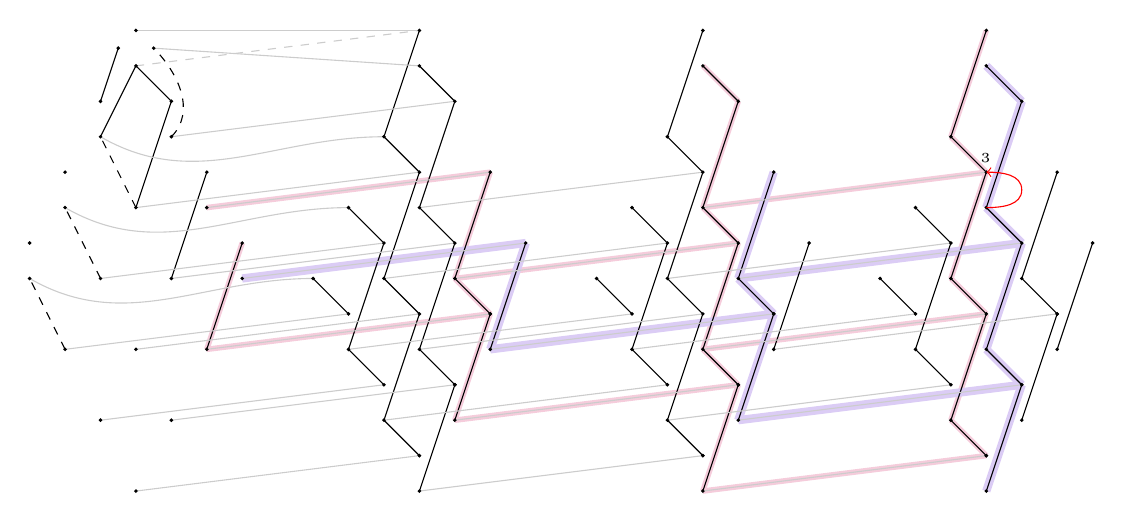
\begin{tikzpicture}[scale=.45]
    % SHADED PART 1
    \foreach \z/\x/\y in {0/5/4, 8/4/2,8/4/6, 16/3/0,16/3/4,16/3/8, 24/2/2,24/2/6,24/2/10}
      {\draw[pretzelshading1] (\x+\z,\y) to (\x+\z+1,\y+3);}
    \foreach \z/\x/\y in {8/5/5, 16/4/3,16/4/7,16/4/11, 24/3/1,24/3/5,24/3/9}
      {\draw[pretzelshading1] (\x+\z,\y) to (\x+\z-1,\y+1);}
    \foreach \z/\x/\y in {8/5/5,8/5/9, 16/4/3,16/4/7, 24/3/1,24/3/5,24/3/9}
      {\draw[pretzelshading1] (\x+\z,\y) to (\x+\z-8,\y-1);}
    % SHADED PART 2
    \foreach \z/\x/\y in {8/5/4, 16/4/2,16/4/6, 24/3/0,24/3/4,24/3/8}
      {\draw[pretzelcol2!20,line width=3pt] (\x+\z,\y) to (\x+\z+1,\y+3);}
    \foreach \z/\x/\y in {16/5/5, 24/4/3,24/4/7,24/4/11}
      {\draw[pretzelcol2!20,line width=3pt] (\x+\z,\y) to (\x+\z-1,\y+1);}
    \foreach \z/\x/\y in {8/6/7, 16/5/5, 24/4/3,24/4/7}
      {\draw[pretzelcol2!20,line width=3pt] (\x+\z,\y) to (\x+\z-8,\y-1);}
    %
    % LINES
    % first square
    \foreach \x/\y in {5/4,4/6,3/8}
      {\draw (\x,\y) to (\x+1,\y+3);}
    \foreach \x/\y in {1/4,2/6,3/8}
      {\draw[dashed] (\x,\y) to (\x-1,\y+2);}
    \draw (2,10) to (3,12);
    \draw (2,11) to (2.5,12.5);
    \draw (4,11) to (3,12);
    \draw[dashed,out=45,in=-45] (4,10) to (3.5,12.5);
    % other squares
    \foreach \z in {8,16,24} {
      \foreach \x/\y in {3/0,2/2,4/2,1/4,3/4,5/4,2/6,4/6,3/8,2/10}
      {\draw (\x+\z,\y) to (\x+\z+1,\y+3);}
      \foreach \x/\y in {3/1,2/3,4/3,1/5,3/5,5/5,2/7,4/7,3/9,4/11}
      {\draw (\x+\z,\y) to (\x+\z-1,\y+1);}
    }
    %
    % INTERSQUARES
    % first intersquare
    \foreach \x/\y in {0/6,1/8,2/10}
      {\draw[draw=black!20,out=-30,in=-180] (\x,\y) to (\x+8,\y);}
    \foreach \x/\y in {6/6,5/8,4/10}
      {\draw[draw=black!20] (\x,\y) to (\x+8,\y+1);}
    \draw[draw=black!20] (3.5,12.5) to ++(7.5,-.5);
    \draw[draw=black!20] (3,13) to ++(8,0);
    \draw[dashed,draw=black!20] (3,12) to ++(8,1);
    % other intersquares
    \foreach \z in {8,16,24} {
      \foreach \x/\y in {3/1,2/3,4/3,1/5,3/5,5/5,2/7,4/7,3/9}
      {\draw[draw=black!20] (\x+\z,\y) to (\x+\z-8,\y-1);}
    }
    %
    % POINTS
    % first square
    \foreach \x/\y in {
      3/0,2/2,4/2,1/4,3/4,5/4,2/6,4/6,3/8,
      0/6,0/7,1/8,1/9,2/10,2/11,
      6/6,6/7,5/8,5/9,4/10,4/11,
      3/12,2.5/12.5,3.5/12.5,3/13
    }
    {\node[fill=black,circle,inner sep=.5pt] at (\x,\y){};}
    % other squares
    \foreach \z in {8,16,24} {
      \foreach \x/\y in {3/1,2/3,4/3,1/5,3/5,5/5,2/7,4/7,3/9,4/11}
      {\node[fill=black,circle,inner sep=.5pt] at (\x+\z,\y){};
      \node[fill=black,circle,inner sep=.5pt] at (\x+\z-1,\y+1){};}
      \foreach \x/\y in {3/0,4/2,5/4,3/1,4/3,5/5,6/7,5/9,3/13}
      {\node[fill=black,circle,inner sep=.5pt] at (\x+\z,\y){};}
    }
    %
    \node[below] at (6,6) {\tiny $\bZ$};
    \node[below] at (12,6) {\tiny $\bZ$};
    \node[below] at (24+3,8) {\tiny $\bZ$};
    \node[above] at (24+3,9) {\tiny $\bZ_3$};
    \draw[red,->] (24+3,8) to[out=0,in=-90] (24+4,8.5) to[out=90,in=0] (24+3,9);
  \end{tikzpicture}
  \caption{A schematic for the hypercube associated to $P(3,3,-3)$. (Dashed) lines are (resp.\ minus) identities between copies of $\bZ$; homological degree goes from left to right. Two connected components are highlighted; labels ``$\bZ$'' and ``$\bZ_3$'' indicate how they contribute to the homology. A red arrow indicates the $\lief$-action induced on homology.}
  \label{subfig:pretzel_3_schematic}
\end{subfigure}

\caption{The proof of \cref{thm:main_pretzel} in the case of $P(3,3,-3)$.}
\label{fig:pretzel_3}
\end{figure}

We aim to show these claims for generic $n\in\bN$.
It is not hard to extend the schematic; the relevant connected components are as follows:
\begin{center}
  \begin{tikzpicture}[scale=.3]
    \tikzset{pretzelshading1/.style={draw=pretzelcol1!20,line width=2pt}}
    \tikzset{pretzelshading2/.style={draw=pretzelcol2!20,line width=2pt}}
    % PART 1
    % big slanted line
    \foreach \x/\y in {
      7/2, 35/10,
      42/-8,42/-4,42/0,42/4,42/8
    }
      {\draw[pretzelshading1] (\x,\y) to (\x+1,\y+3);}
    % marked big slanted line
    \foreach \x/\y in {
      0/0, 7/-2, 14/-4,14/0,14/4,
      21/-6,21/-2,21/2,21/6, 28/-8,28/-4,28/0,28/4,28/8,
      35/-10,35/-6,35/-2,35/2,35/6,
      42/12
    }
      {\draw[pretzelshading1] (\x,\y) to node[gaussmark] {} (\x+1,\y+3);}
    %
    % small slanted line
    \foreach \x/\y in {
      0/0, 7/-2,7/2, 14/-4,14/0,14/4,
      21/-6,21/-2,21/2,21/6, 28/-8,28/-4,28/0,28/4,28/8,
      35/10
    }
      {\draw[pretzelshading1] (\x+8,\y+1) to (\x-1+8,\y+1+1);}
    % marked small slanted line
    \foreach \x/\y in {
      28/12,
      35/-10,35/-6,35/-2,35/2,35/6
    }
      {\draw[pretzelshading1] (\x+8,\y+1) to node[gaussmark] {} (\x-1+8,\y+1+1);}
    %
    % connecting lines
    \foreach \x/\y in {
      0/0, 7/-2,7/2, 14/-4,14/0,14/4,
      21/-6,21/-2,21/2,21/6,
      28/-8,28/-4,28/0,28/4,28/8,
      35/-10,35/-6,35/-2,35/2,35/6,35/10,
      0/4
    }
      {\draw[pretzelshading1] (\x,\y) to (\x+8,\y+1);}
    % marked connecting lines
    \foreach \x/\y in {
      0/4
    }
      {\draw[pretzelshading1] (\x,\y) to node[gaussmark] {} (\x+8,\y+1);}
    %
    % PART 2
    \begin{scope}[shift={(1,-2)}]
      % big slanted line
      \foreach \x/\y in {
        42/12
      }
        {\draw[pretzelshading2] (\x,\y) to (\x+1,\y+3);}
      % marked big slanted line
      \foreach \x/\y in {
        7/2, 14/0, 21/-2, 28/-4, 35/-6,
        14/4,
        21/2,21/6, 28/0,28/4,28/8,
        35/-2,35/2,35/6,35/10,
        42/-8,42/-4,42/0,42/4,42/8
      }
        {\draw[pretzelshading2] (\x,\y) to node[gaussmark] {} (\x+1,\y+3);}
      %
      % small slanted line
      \foreach \x/\y in {
        7/2, 14/0,14/4,
        21/-2,21/2,21/6, 28/-4,28/0,28/4,28/8,
        35/-6,35/-2,35/2,35/6,35/10
      }
        {\draw[pretzelshading2] (\x+8,\y+1) to (\x-1+8,\y+1+1);}
      % marked small slanted line
      \foreach \x/\y in {
        35/14
      }
        {\draw[pretzelshading2] (\x+8,\y+1) to node[gaussmark] {} (\x-1+8,\y+1+1);}
      %
      % connecting lines
      \foreach \x/\y in {
        0/4, 7/2, 14/0, 21/-2, 28/-4, 35/-6,
        14/4,
        21/2,21/6,
        28/0,28/4,28/8,
        35/-2,35/2,35/6,35/10,
        0/4
      }
        {\draw[pretzelshading2] (\x,\y) to (\x+8,\y+1);}
    \end{scope}
    %
    \node[circle,fill=pretzelcol1!50,inner sep=2pt] (A1) at (7,2) {};
    \node[below left={-5pt}of A1] {\footnotesize $A$};
    \node[circle,fill=pretzelcol1!50,inner sep=2pt] (A2) at (35,10) {};
    \node[left={-3pt}of A2] {\footnotesize $B$};
    \node[circle,fill=pretzelcol1!50,inner sep=2pt] (A3) at (43,11) {};
    \node[right={-3pt}of A3] {\footnotesize $C$};
    \node[circle,fill=pretzelcol2!50,inner sep=2pt] (B) at (43,10) {};
    \node[right={-3pt}of B] {\footnotesize $D$};
    \node[circle,fill=pretzelcol2!50,inner sep=2pt] (E) at (1,2) {};
    \node[right={-3pt}of E] {\footnotesize $E$};
    \draw[pretzelcol1!50,line width=2pt] (A1) to[out=45,in=165] node[black,above=-1pt,pos=.2]{\footnotesize $n$} (A3);
    \draw[pretzelcol1!50,line width=2pt] (A2) to[out=45,in=165] node[black,above=-1pt,pos=.12]{\footnotesize $n$}(A3);
    \foreach \x/\y in {
      14/0,21/-2,28/-4,28/-8,35/-10,
      42/-8,42/-4,42/0,42/4,42/8
    }
      {\draw[thick,dashed] (\x,\y) to (\x+1,\y+3);}
    \foreach \x/\y in {
      28/-4,
      42/-8,42/-4,42/0,42/4,42/8
    }
      {\draw[thick,dashed] (\x,\y) to (\x+1,\y-1);}
    \foreach \x/\y in {
      7/2,14/0,21/-2,28/-8,35/-10
    }
      {\draw[thick,dashed] (\x,\y) to (\x+8,\y+1);}
  \end{tikzpicture}
\end{center}
We perform gaussian elimination on the arrows marked with $\tikzpic{\node[circle,fill=white,draw=black,line width=1pt,inner sep=3pt] at (0,0){};}$ .
The only surviving vertices are $A$, $B$, $C$, $D$ and $E$, as depicted. Moreover, this happens away from $C$ and $D$, and hence leaves the action of $\lief$ from $C$ to $D$ unaffected.
Gaussian elimination may induce maps between these vertices; to find these maps, one must compute the number of paths between two vertices, alternating between marked and unmarked edges.
For the blue connected component, no such path exists, and so $D$ and $E$ each contribute with a copy of $\bZ$ to homology.

There are paths from $B$ to $C$; they consist in going down a certain number of steps, then right, then up the same number of steps. This makes $n$ such paths.
Similarly, there are $n$ paths from $A$ to $C$, consisting of going down-right the second-to-last ``stair'' a certain number of steps, then going down, then going down-right the last ``stair'' until reaching the bottom-right, and finally going up to $C$; one of such paths is depicted in dashed lines.
Computing homology will (say) kill the vertex $B$ and make $C$ a copy of $\bZ/n\bZ$; the arrow from $A$ to $C$ is then zero, leaving $A$ to contribute with a copy of $\bZ$ to homology.

This concludes the proof of \cref{thm:main_pretzel}.